\documentclass{tufte-handout}
% \documentclass{article}

%\date{28 March 2010} % without \date command, current date is supplied

% \geometry{showframe} % display margins for debugging page layout

\usepackage{graphicx} % allow embedded images
  \setkeys{Gin}{width=\linewidth,totalheight=\textheight,keepaspectratio}
  \graphicspath{{graphics/}} % set of paths to search for images
\usepackage{amsmath}  % extended mathematics
\usepackage{booktabs} % book-quality tables
\usepackage{units}    % non-stacked fractions and better unit spacing
\usepackage{multicol} % multiple column layout facilities
\usepackage{lipsum}   % filler text
\usepackage{fancyvrb} % extended verbatim environments
  \fvset{fontsize=\normalsize}% default font size for fancy-verbatim environments
\usepackage{listings}

% Standardize command font styles and environments
\newcommand{\doccmd}[1]{\texttt{\textbackslash#1}}% command name -- adds backslash automatically
\newcommand{\docopt}[1]{\ensuremath{\langle}\textrm{\textit{#1}}\ensuremath{\rangle}}% optional command argument
\newcommand{\docarg}[1]{\textrm{\textit{#1}}}% (required) command argument
\newcommand{\docenv}[1]{\textsf{#1}}% environment name
\newcommand{\docpkg}[1]{\texttt{#1}}% package name
\newcommand{\doccls}[1]{\texttt{#1}}% document class name
\newcommand{\docclsopt}[1]{\texttt{#1}}% document class option name
\newenvironment{docspec}{\begin{quote}\noindent}{\end{quote}}% command specification environment

\begin{document}

\title{MAE-253: Homework 1}
\author[John Karasinski]{John Karasinski}
\maketitle% this prints the handout title, author, and date

\section{Problem 1}

\begin{marginfigure}%
  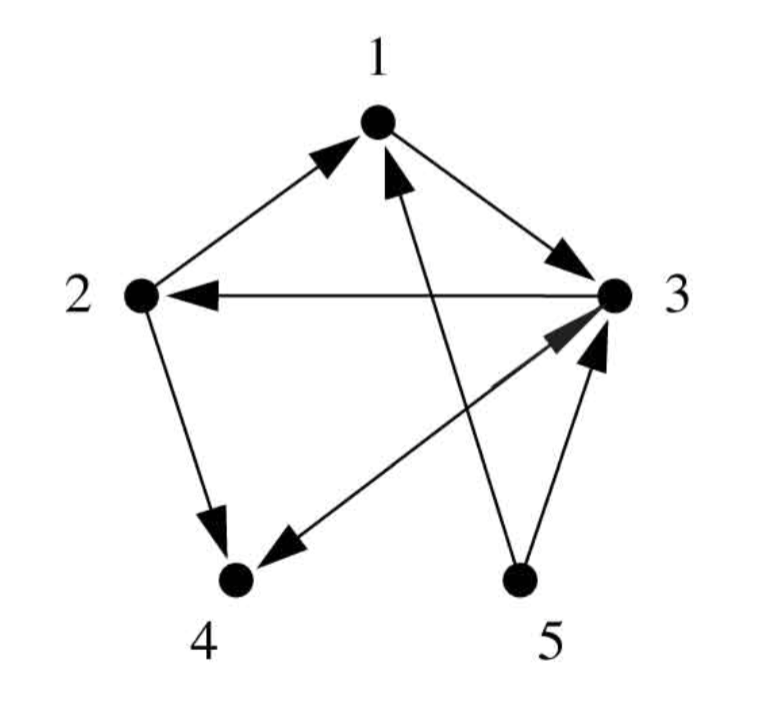
\includegraphics[width=\linewidth]{../graph.png}
  \caption{Simple network.}
  % \label{fig:marginfig}
\end{marginfigure}

\subsection{a)
Consider the simple network shown above and write down its the adjacency matrix.}

\begin{align*}
A =
\begin{bmatrix}
  0 & 1 & 0 & 0 & 1 \\
  0 & 0 & 1 & 0 & 0 \\
  1 & 0 & 0 & 1 & 1 \\
  0 & 1 & 1 & 0 & 0 \\
  0 & 0 & 0 & 0 & 0 \\
\end{bmatrix}
\end{align*}

\subsection{b)
Consider a random walk on this network. What is the steady-state probability of finding the walker on each node?}

To find the stead-state probability of finding a random walker on any node, we first calculate the transition matrix by normalizing $A$ column-wise.
\begin{align*}
T =
\begin{bmatrix}
0 & 0.5 &  0   &  0 & 0.5 \\
0 & 0   &  0.5 &  0 & 0   \\
1 & 0   &  0   &  1 & 0.5 \\
0 & 0.5 &  0.5 &  0 & 0   \\
0 & 0   &  0   &  0 & 0   \\
\end{bmatrix}
\end{align*}
The steady-state probability is the eigenvector of $T$ associated with the eigenvalue of 1,
\begin{align*}
\pi =
\begin{bmatrix}
-0.18257419 \\
-0.36514837 \\
-0.73029674 \\
-0.54772256 \\
 0          \\
\end{bmatrix}.
\end{align*}
Normalizing $\pi$, we have
\begin{align*}
\pi =
\begin{bmatrix}
0.1 \\
0.2 \\
0.4 \\
0.3 \\
0 \\
\end{bmatrix}.
\end{align*}

\subsection{c)
What would be the steady-state probability of finding the walker on each node if the edges were instead undirected?}

The steady-state probability of finding a walker on a node of an undirected graph is the degree of the node divided by the total number of edges,
\begin{align*}
\pi = \dfrac{1}{14}
\begin{bmatrix}
3 \\
3 \\
4 \\
2 \\
2 \\
\end{bmatrix}.
\end{align*}


% \lstinputlisting[language=Python]{../homework1.py}
% \vspace{5em}

\section{Problem 2}
Consider a variant of the BA model that does not feature preferential attachment.
We start with a single node at time $t = 1$. In each subsequent discrete time step, a
new node is added with $m = 1$ links to existing nodes. The probability that a link
arriving at time step $t + 1$ connects to any existing node $i$ is uniformly distributions
and independent of $i$:
\begin{align*}
\pi_i = \dfrac{1}{t}.
\end{align*}
Let $n_{k,t}$ denote the expected number of nodes of degree $k$ at time $t$. For the steps below, proceed as in lecture.

\subsection{a)
Write the rate equation for $n_{k,t+1}$ in terms of the $n_{j,t}$'s. (Note you will need to equations, one for $k = 1$ and one for $k > 1$.)}

\begin{align*}
k = 1; \hspace{2em} & n_{1,t+1} = n_{1,t} + 1 - \dfrac{1}{t} n_{1,t} \\
k > 1; \hspace{2em} & n_{k,t+1} = n_{k,t} + \dfrac{1}{t}n_{k-1,t} - \dfrac{1}{t} n_{k,t}
\end{align*}

\subsection{b)
Converting from expected number of nodes to probabilities, $p_{k,t} = n_{k,t}/n_t$, rewrite the equations in part (a) in terms of the probabilities.}

\begin{align*}
p_{k,t} = n_{k,t}/n_t \implies n_{k,t} =& p_{k,t} n_t \\
                                       =& p_{k,t} \cdot t
\end{align*}
From a), we then have
\begin{align*}
k = 1; \hspace{2em} & p_{1,t+1} (t+1) = p_{1,t} + 1 - \dfrac{1}{t} p_{1,t} \cdot t \\
k > 1; \hspace{2em} & p_{k,t+1} (t+1) = p_{k,t} \cdot t + \dfrac{1}{t} p_{k-1,t} \cdot{t} - \dfrac{1}{t} p_{k,t} \cdot{t}
\end{align*}

\subsection{c)
Assume steady-state, that $p_{k,t} = p_{k}$, and solve the recurrence relation to obtain $p_k$ in terms of $p_{k-1}$.}

\begin{align*}
k > 1; \hspace{2em} & p_{k} (t+1) = p_{k} \cdot t + \dfrac{1}{t} p_{k-1} \cdot{t} - \dfrac{1}{t} p_{k} \cdot{t} \\
                    & p_{k} (t+1) = p_{k} (t - 1) + \dfrac{1}{t} p_{k-1} \\
                    & p_{k} (t+1-t+1) = \dfrac{1}{t} p_{k-1} \\
                    & p_{k} = \dfrac{1}{2} p_{k-1} \\
\end{align*}

\subsection{d) Starting by solving for $p_1$ and recursing, derive the expression for the stationary degree distribution $p_k$.}
\begin{align*}
k = 1; \hspace{2em} & p_{1} (t+1) = p_{1} + 1 - \dfrac{1}{t} p_{1} \cdot t \\
                    & p_{1} (t+1) = 1 \\
                    & p_{1} = \dfrac{1}{2} \\
\end{align*}
Plugging this into our equation for $p_{k}$, we find the following relation:

\begin{align*}
p_{k} = \left( \dfrac{1}{2} \right)^k
\end{align*}


% \begin{marginfigure}%
%   \includegraphics[width=\linewidth]{helix}
%   \caption{This is a margin figure.  The helix is defined by
%     $x = \cos(2\pi z)$, $y = \sin(2\pi z)$, and $z = [0, 2.7]$.  The figure was
%     drawn using Asymptote (\url{http://asymptote.sf.net/}).}
%   \label{fig:marginfig}
% \end{marginfigure}

% \begin{figure*}[h]
%   \includegraphics[width=\linewidth]{sine.pdf}%
%   \caption{This graph shows $y = \sin x$ from about $x = [-10, 10]$.
%   \emph{Notice that this figure takes up the full page width.}}%
%   \label{fig:fullfig}%
% \end{figure*}

% \begin{figure}
%   \includegraphics{hilbertcurves.pdf}
% %  \checkparity This is an \pageparity\ page.%
%   \caption{Hilbert curves of various degrees $n$.
%   \emph{Notice that this figure only takes up the main textblock width.}}
%   \label{fig:textfig}
%   %\zsavepos{pos:textfig}
%   \setfloatalignment{b}
% \end{figure}

\end{document}
